\documentclass[11pt,oneside,letterpaper]{article}

% graphicx package, useful for including eps and pdf graphics
\usepackage{graphicx}
\DeclareGraphicsExtensions{.pdf,.png,.jpg}

% basic packages
\usepackage{color}
\usepackage{parskip}
\setlength{\parskip}{0.15cm}
\usepackage{float}
\usepackage{todonotes}
\usepackage{enumitem}
\usepackage{microtype}
\usepackage{url}
\urlstyle{same}

% text layout
%\usepackage[left=0.6in,right=0.6in,top=0.5in,bottom=0.6in,footskip=0.7in]{geometry}
\usepackage[letterpaper,margin=0.6in,footskip=0.7in]{geometry}
\pagestyle{empty}

% section titles
\usepackage[compact]{titlesec}
\titleformat{\subsubsection}[runin]{\normalfont\bfseries}{\thesubsubsection}{3pt}{}[ $\;\cdotp\;$]
\titlespacing{\subsubsection}{0pt}{*1}{*0.5}

% helps to keep figures from being orphaned on a page by themselves
\renewcommand{\topfraction}{0.85}
\renewcommand{\textfraction}{0.1}

% bold the 'Figure~#' in the caption and separate it with a period
% captions will be left justified
\usepackage[labelsep=period,font=small,labelfont=bf]{caption}

% defining paragraph tabs
\newcommand\tab[1][1cm]{\hspace*{#1}}

% cite package, to clean up citations in the main text. Do not remove.
\usepackage{cite}

% remove brackets from numbering in list of References
\renewcommand\refname{Bibliography and References Cited}
\makeatletter
\renewcommand{\@biblabel}[1]{\quad#1.}
\makeatother

% authors
\usepackage{authblk}
\renewcommand\Authands{ \& }
\renewcommand\Authfont{\normalsize \bf}
\renewcommand\Affilfont{\small \normalfont}
\makeatletter
\renewcommand\AB@affilsepx{, \protect\Affilfont}
\makeatother

% notation
\usepackage{amsmath}
\usepackage{amssymb}
\usepackage{bbm}

%%% TITLE %%%
\title{\vspace{1.0cm} \LARGE \bf Estimating phylogenetic placement of unsampled infections}

\author[1]{Stephanie Stacy}
\author[1,2]{Allison Black}
\author[1]{Gytis Dudas}
\author[1]{Trevor Bedford}

\affil[1]{Vaccine and Infectious Disease Division, Fred Hutchinson Cancer Research Center, Seattle, WA, USA}
\affil[2]{Department of Epidemiology, University of Washington, Seattle, WA, USA}


\date{\today}

\begin{document}

%% TITLE
\maketitle

%% ABSTRACT
\begin{abstract}


\end{abstract}

\pagebreak

%% INTRODUCTION
\section*{Introduction}


%% MODEL
\section*{Model}
\subsection*{Applying the Coalescent Framework}
\tab The standard coalescent is a stochastic process modeling the genealogy of a given set of samples within a larger population. When trees of samples are created under this framework, waiting times between coalescent events -- events where lineages find their most recent common ancestor (MRCA) -- have a known distribution. With an existing idea of how samples are likely to be distributed within a phylogenetic tree, we can calculate a probability of a new unknown sequence attaching to each existing branch in that tree. 

\tab We focus on the simplest form of Kingman's model of coalescence () with a constant population size across time and selectively neutral genetic variation. Generations are treated as non-overlapping and the model does not allow for recombination. Under this model, we walk back in time from the present, and the probability two of the total available lineages share a common ancestor a specific number of generations ago follows a geometric distribution in discrete time which approaches an exponential distribution in continuous time. 

\tab To find the most likely place a new, unknown sample coalesces to an existing tree, we begin by assuming a starting tree genealogy, relating $n$ known samples, represents the true relationship between them. We also assume a constant, known effective population size. Unless otherwise specified, a new unknown sequence is treated as if it is sampled at the same time as the most recent tip, and our focus is on evaluating where it is most likely to attach within the existing genealogy.  Assuming the new sample is taken at the same time as the most recent tip provides a heuristic for finding clades that are presently the most likely candidates for undersampling. However, this model also provides attachment probabilities for a sampling event that takes place at a specified time slice anywhere along the tree. 

\subsection*{Conceptualizing Trees as Intervals}
\tab The probability of coalescence depends on the underlying structure of the tree, including the number of available lineages to attach to at any point within the tree. Sampling events may occur at different times; in order to keep track of the number of available lineages at any point in the tree, we record the occurrence of both coalescent events and sampling events. The tree is partitioned into intervals based on these events. 

\tab A tree has $L$ total intervals, $\textbf{i} = \{1, 2, 3, \dots, L\}$, where an increasing index indicates moving backward in time from the tips and the start of the most recent interval is the most recently sampled tip. From the exponentially distributed expectation of coalescence, the probability of coalescence within interval $i$ is
\begin{equation} \label{eq_1}
	P\{coal\} = 1-e^{\frac{-k_it_i}{N}},
\end{equation}
which depends on $N$, the constant effective population size; $k_i$, the number of lineages active within interval $i$; and $t_i$, the length of the interval. Figure \ref{F-intervals} provides an example genealogy with intervals and corresponding lengths and lineages within them.

\begin{figure}[h]
 \centering
	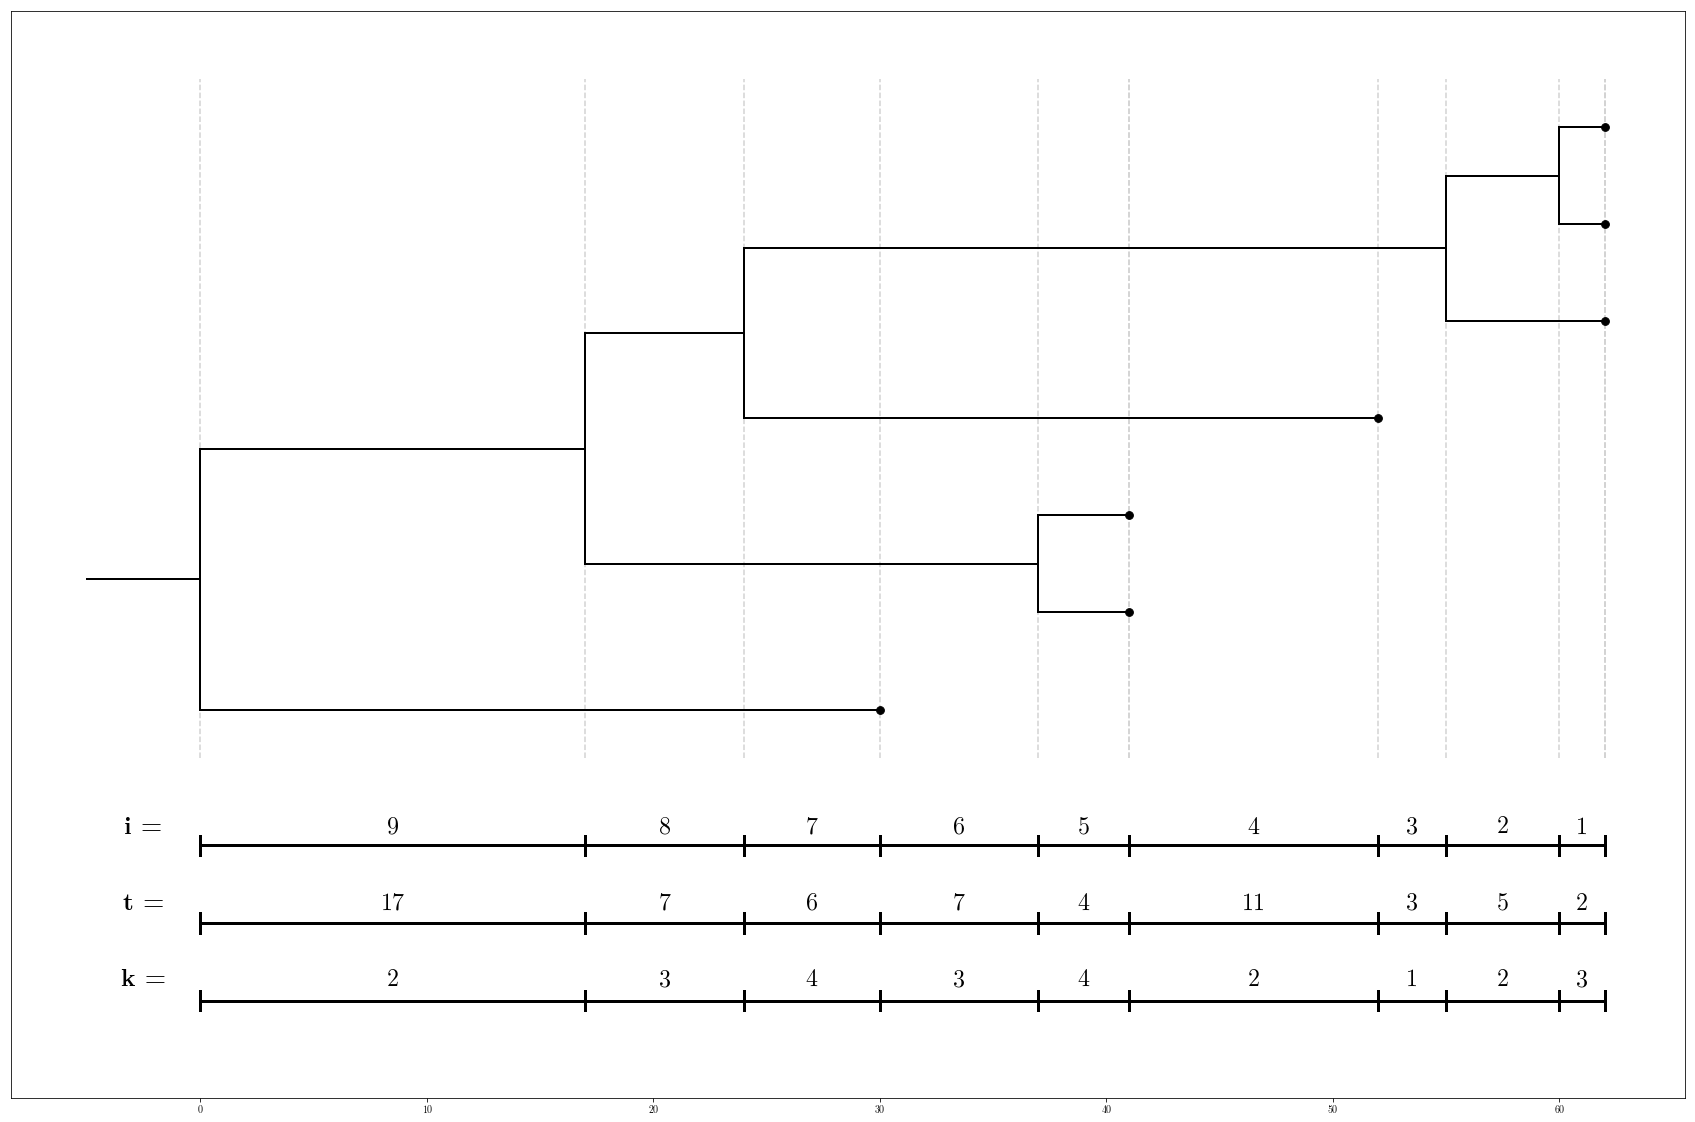
\includegraphics[width=0.75\textwidth]{figures/toy-intervals}
	\caption{\textbf{Example genealogy with notation.}
	Example tree with seven samples and a constant, known population of $N=50$. Sampling and coalescent events are marked by light grey dashed lines. Below we show interval boundaries along with $\textbf{i}$, the index for each interval, $\textbf{t}$, a vector of interval lengths, and $\textbf{k}$, the vector containing number of lineages in each interval.
	}
	\label{F-intervals}
\end{figure}

\subsection*{Conditional Probabilities of Attachment}
\tab Population size, length of interval, and number of available lineages drive the probability of coalescence within each interval, but fail to take into account the difference in time from the unknown sample to each interval within the tree. The probability of a sample coalescing in a specific interval given a sample time incorporates the the temporal distance from the interval to the sample. Temporal distance is accounted for by using the probability of coalescing in an interval conditioned on not coalescing in another, more recent interval. Intuitively, when all other variables are equal, intervals closer in time to the missed sampling event should be more likely candidates for coalescent because the probability that no coalescent event has already occurred decreases with each interval step back in time. However, time from sample, number of lineages, and interval lengths compete against each other to drive probability of coalescence in this equation. If an interval length is large enough, it can offset the effect of temporal distance. The conditional probability of coalescing in interval $i$ becomes
\begin{equation} \label{eq_2}
	P_i = [1-e^{\frac{-k_it_i}{N}}] \cdot \prod_{j=1}^{i-1} e^{\frac{-k_jt_j}{N}},
\end{equation}
where, again, $\bf{t}$ is the vector of $L$ interval lengths and $\bf{k}$ is the vector of the number of lineages in each of the intervals. To find the probability of the sample attaching to a specific branch $b$, simply sum the probabilities of attachment within the interval the branch spans. This results in

\begin{equation} \label{eq_3}
	\Pi_b = \sum_{i=1}^L \mathbbm{1}_i(b) \cdot \frac{1}{k_i}\cdot P_i,
\end{equation}
where $\mathbbm{1}_i(b)$ is an indicator function for whether the branch is present in the current interval. The probability of coalescing beyond the root of the tree is simply one minus the sum of all the other branch probabilities in the tree. The sum of attachment probabilities across the entire set of branches, including the root, must be one, so any probability not accounted for in the other branches of the tree must belong in the root. 

\begin{figure}[h]
 \centering
	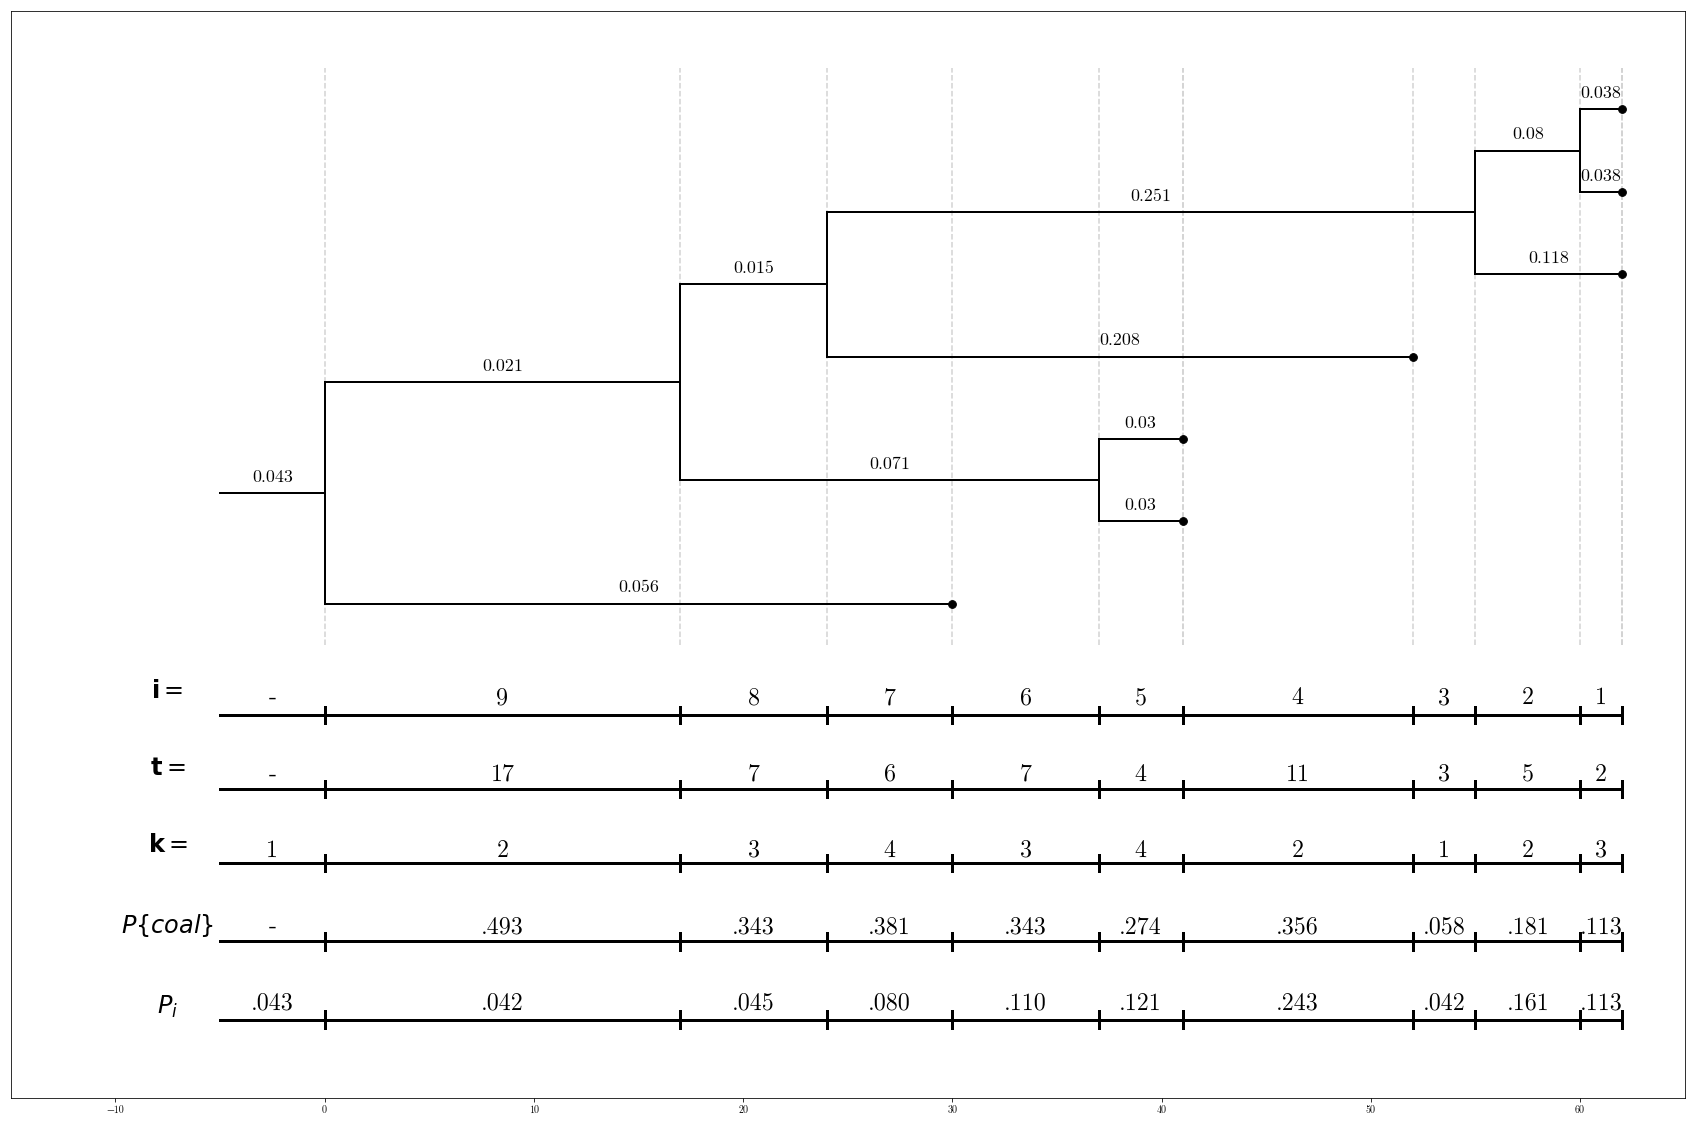
\includegraphics[width=0.75\textwidth]{figures/conditional-pcoal}
	\caption{\textbf{Example genealogy with branch attachment probabilities for an unknown sample.}
	Example tree with seven samples and a constant, known population of $N=50$. Information from equation Fig. \ref{F-intervals} is included as well as the probability of coalescing in each interval, $P\{coal\}$, from Eq. (\ref{eq_1}) and conditional probability of coalescence within an interval, $P_i$, from Eq. (\ref{eq_2}). Each branch is labeled with $\Pi_b$, the probability of attaching to a specific branch from Eq. (\ref{eq_3}). The effect of time on coalescence can be seen when interval 4 is compared to interval 9. Even though they have the same number of lineages and interval 9 is longer, the conditional probability of attaching at interval 9 is smaller due to the distance between sample and that interval.
	}
	\label{F-conditional-pcoal}
\end{figure}
\subsection*{Attachment Probabilities for Time-Sliced Trees}
\tab If a time other than the sampling time of the most recent tip is specified, an unknown sample will be evaluated from that time, effectively slicing the tree at that point. We can then calculate the probabilities of attachment to each branch in the tree in relation to that time slice. Any lineages in intervals that occur more recently than the specified time have no probability of attachment in those intervals. New conditional probabilities are calculated in relation to the time slice with Eq. (\ref{eq_2}). The slice is treated as the most recent possible time and the tree is evaluated starting from time slice and moving back to the root. If the time slice falls within an interval and not at an interval endpoint, the fraction of the interval later than the slice is considered available for attachment.
 
\begin{figure}[h]
 \centering
	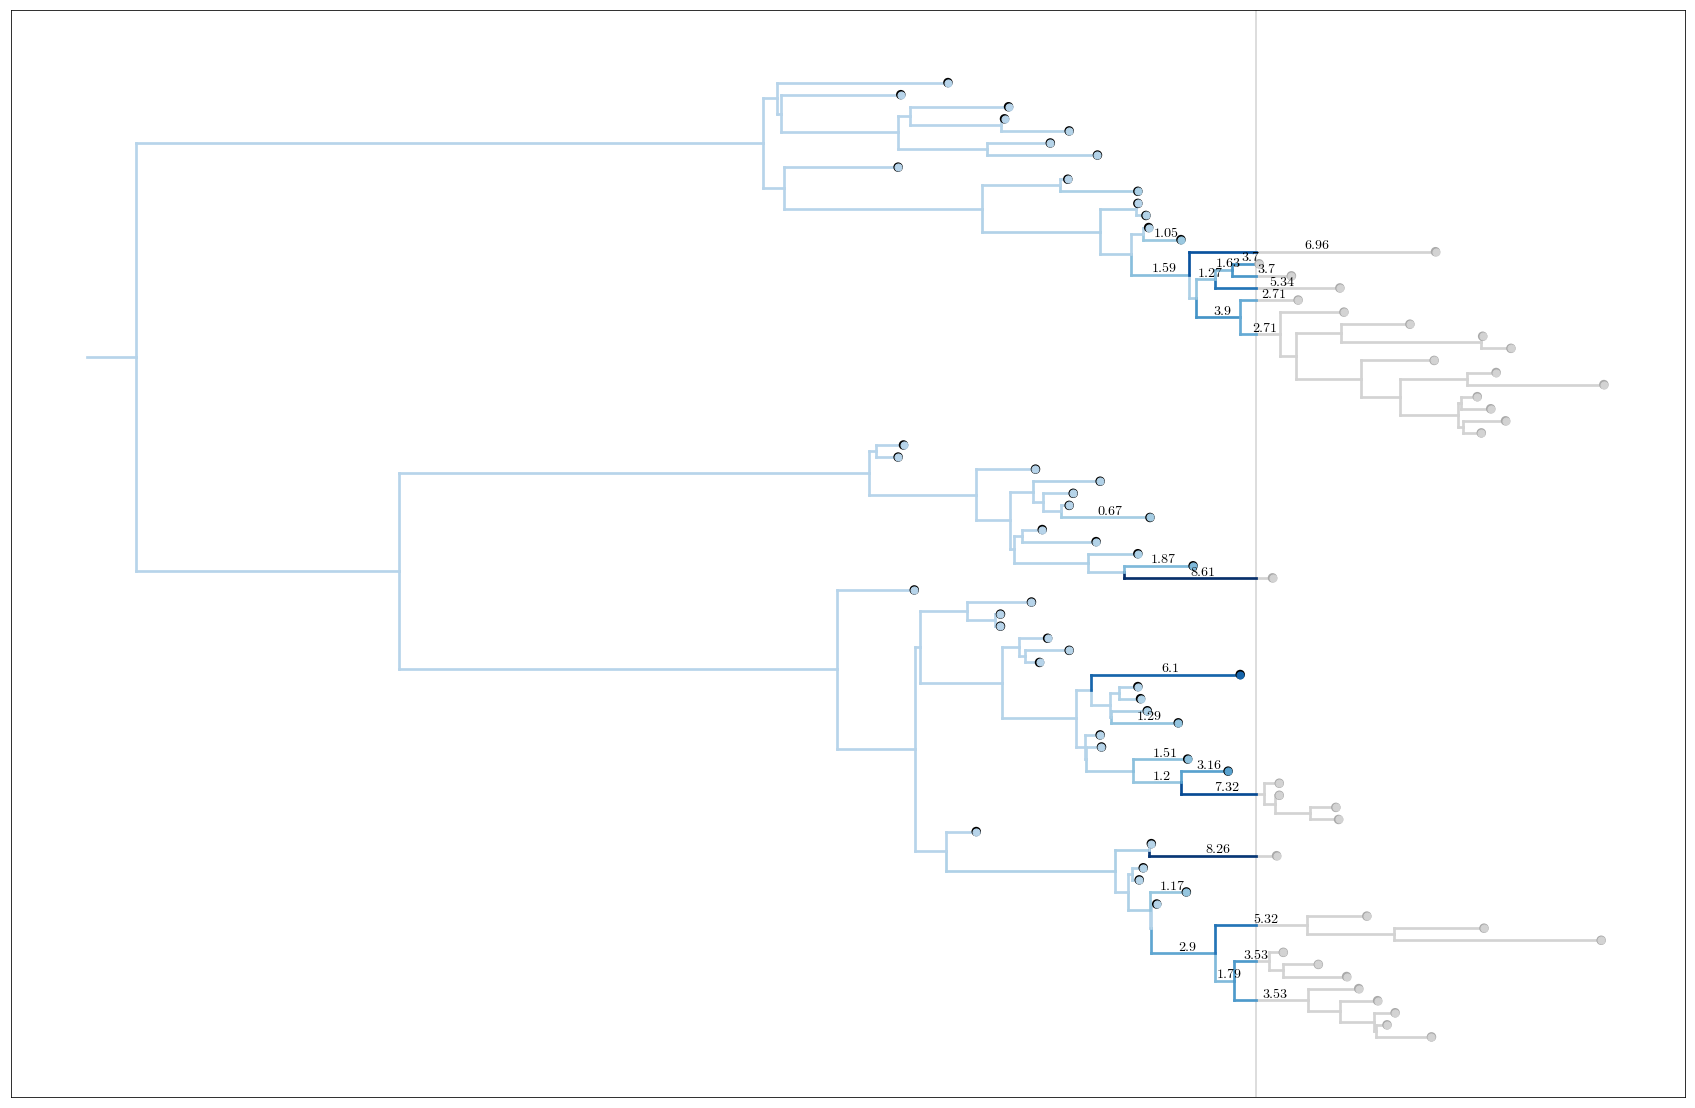
\includegraphics[width=0.75\textwidth]{figures/time-slice}
	\caption{\textbf{Time-sliced tree.}
	Example tree created from a sample of simulated Ebola data. Time slice indicated by the grey, vertical line and corresponds to December 2014 in the Ebola virus outbreak. All branches to the right of the slice are not considered as candidates for attachment and a new, unknown sequence is considered at the time slice. The tree is evaluated from the slice to the root of the tree. Branches are labeled with their probability of attachment expressed as a percentage. Only branches with at least a 1\% chance of attachment are labeled.
	}
	\label{F-time-slice}
\end{figure}

\tab In most cases, we would be interested in looking at attachment probabilities from a time slice somewhere in the existing tree, however, it is also possible to set a slice outside this range. A new sample added at a time further back than the root will coalesce to the root with probability 1 as it has no other available lineages. A new sample added more recently than the most recent existing sample is treated the same as if the new sample was added at the time of the most recent tip, except an interval from the unknown sample to the most recent existing sample is added with no possibility for attachment.

\subsection*{Expected Sampling Proportion Along the Full Tree}
\tab It is simple to move from the addition of a single, unknown sample to the total distribution of expected sampling across the tree. Under any clade  $c$ in the tree, the sum of $\Pi_b, \forall b \in c$ represents the probability of a single sample coalescing under that clade. Equivalently, this is the proportion of total unknown samples, sampled at that time point, expected to fall under that clade. Here, we move from where a single new sample is expected to attach to how much of the total sampling we should see within each clade. These proportions are cumulative, and each clade contains the proportion of sampling expected in all of its nested clades in addition to that of unique branches. Figure \ref{F-cumulative-node-prob} gives an illustration of what this looks like.

\begin{figure}[h]
 \centering
	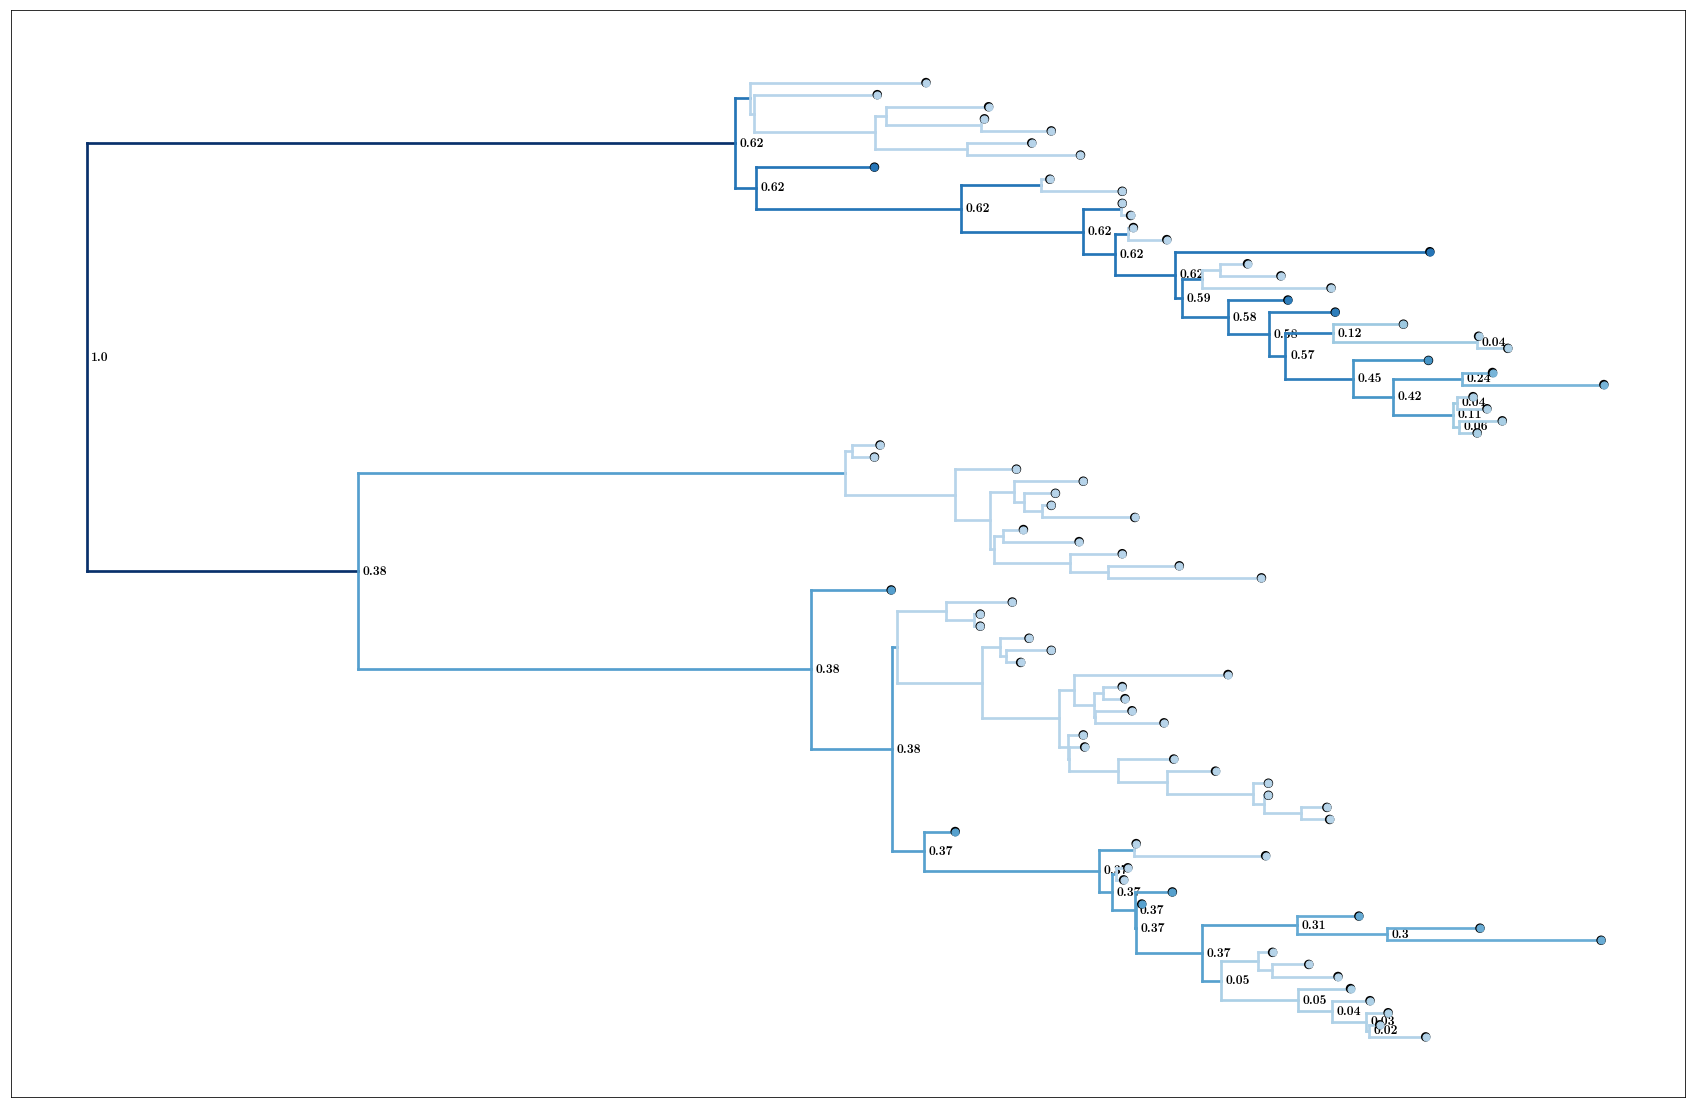
\includegraphics[width=0.75\textwidth]{figures/cumulative-clade-prop}
	\caption{\textbf{Expected cumulative proportion of sampling under each node.}
	Example tree created from a sample of simulated Ebola data. Darker blue represents a greater proportion of sampling expected within the clade. Clades with at least 1\% of total expected sampling are labeled.
	}
	\label{F-cumulative-node-prob}
\end{figure}

\tab An idea about how sampling is expected to be distributed under the coalescent framework is the first step toward targeting undersampled clades. We expect good candidates for undersampled pockets to occur where the actual observed sampling is much less than expected from the coalescent. However, finding absolute differences between observed and expected sampling is not enough. We are interested in whether this difference is meaningful in the context of the tree and, for practical purposes, prioritize a select few pockets representing areas of greatest expected missing samples. 

\tab We use z-scores, a measure for normalization, to determine which differences deviate most from expected. Differences are calculated by finding the difference between the expected cumulative sampling proportion, explained in the preceding paragraph, and the number of samples actually observed under the clade divided by the total $n$ samples in the genealogy. Each internal node in the tree is given a difference score. The set of all difference scores are normalized to have mean zero, standard deviation one. Any node with a z-score of magnitude greater than two is traditionally consider outlying. In this case, large, positive z-scores represent the most likely candidates of undersampling.

\begin{figure}[h]
 \centering
	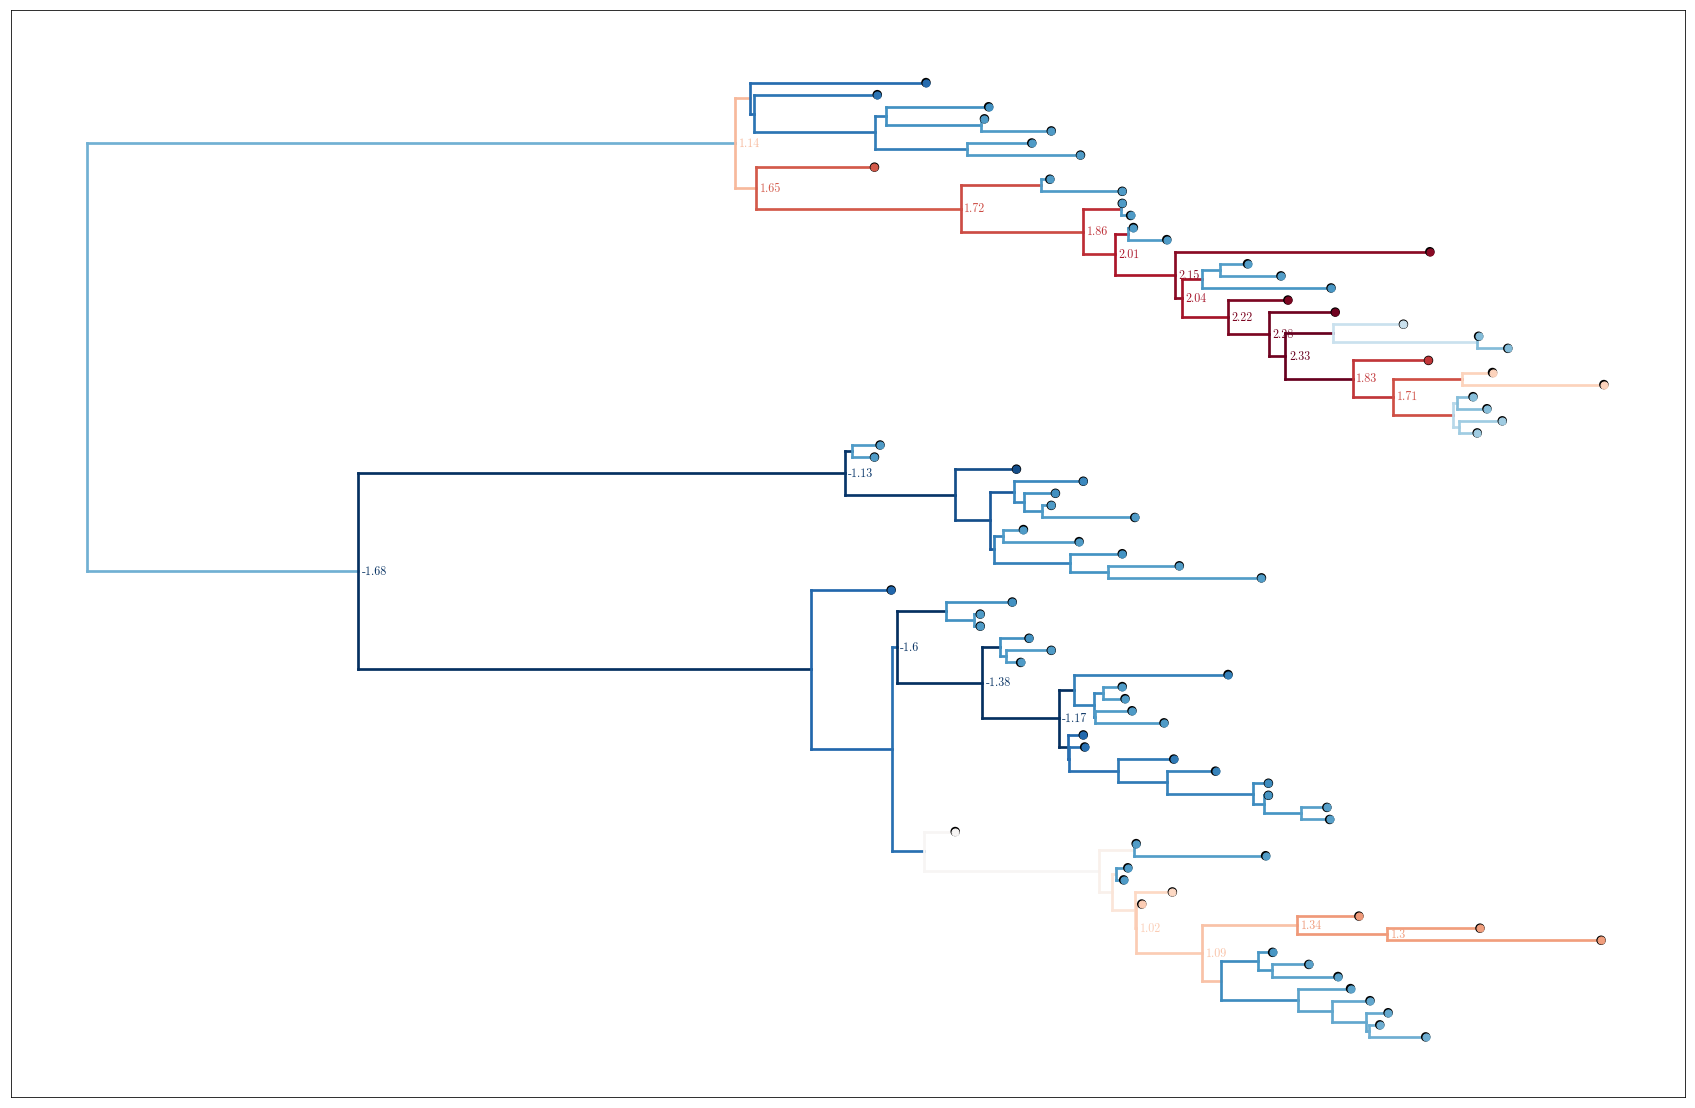
\includegraphics[width=0.75\textwidth]{figures/z-scores}
	\caption{\textbf{Z-scores along example tree.}
	Example tree created from a sample of simulated Ebola data. Color corresponds to z-score where darker blue are large negative z-scores and dark red are large positive ones. Areas of darker red indicate possible candidates for undersampling.
	}
	\label{F-z-scores}
\end{figure}

%% RESULTS
\section*{Results}
\subsection*{Model Performance on Simulated Data}
\tab We examine the ability of our model to correctly predict where, along an existing genealogy, unknown samples are most likely to attach. For five simulated Ebola virus tree genealogies that adhere to the coalescent framework, we feed our model a pruned tree consisting of 5\% (161) of the samples. Sampling times for the remaining 95\% (1,449) of samples are retained and given to the model as time slices. We then find each dropped sample's probability of attachment to each branch in the pruned tree. We measure performance against the true full tree as well as relative performance to other models. Both error on a sample by sample basis and differences between overall expected and observed sample distribution, measured both qualitatively and quantitatively, are assessed.

\tab Model performance on a sample-specific level is determined by categorical cross-entropy, a measure of node impurity within a tree. Given a sample's distribution of branch by branch expected attachment probabilities, this measure penalizes more heavily for low expected probability of samples coalescing at the correct branch. Predicting the correct branch a sample attaches to with probability 1 leads to no penalty for the sample. When the tree structure fulfills coalescent assumptions, the attachment probabilities calculated by our coalescent-based framework consistently outperform two null models, representing neutral attachment preferences.

\begin{table}[h]
\centering
\begin{tabular}{cccc}
\hline
Tree & Coalescent & Null 1 & Null 2\\ \hline
1    & 3.419     & 5.069 & 4.980\\
2    & 3.929     & 5.069 & 5.129 \\
3    & 3.814    & 5.069 & 5.203 \\
4    & 3.264   & 5.069 & 4.767 \\
5    & 3.827     & 5.069 & 4.872 \\ \hline
\end{tabular}
\caption{\textbf{Model Performance Comparison Across Simulated Trees.}
	The average per sample cross-entropy for the model built with the coalescent framework compared to Null 1, a null model where the probability of attachment to each branch is equal and Null 2, the null model where the probability of attachment to each place in the tree is equal. Performance scores were tabulated for five simulated pruned trees.
	}
\label{t-entropy}
\end{table}

\tab If instead of sample-specific performance, we are interested in the overall distribution of expected attachments to each branch, we can sum the probabilities of attachment to a specific branch across all samples. This represents the total number expected to attach to branch $b$ out of all dropped samples. Correlation between the number of expected and observed dropped samples attach to each branch within the pruned tree gives an overall quantitative measure of performance. If the model were performing perfectly, we would expect a correlation coefficient of 1. We observe a moderate to high positive linear relationship between observed and expected samples on a branch. Table \ref{t-correlations} gives the calculated correlation coefficient for each of the five simulated trees. Additionally, Fig. \ref{F-corr} plots an example of the branch by branch comparison between expected and observed attachments for one of the five trees.

\begin{table}[]
\centering
\begin{tabular}{cc}
\hline
Tree & Correlation \\ \hline
1    & 0.627       \\
2    & 0.652       \\
3    & 0.668       \\
4    & 0.793       \\
5    & 0.702       \\ \hline
\end{tabular}
\caption{\textbf{Correlation between expected and observed attachments.} 
The correlation between the number of samples observed to attach to each branch in the pruned tree against the aggregated number of dropped samples expected to attach to the same branch, calculated for each of the five trees. In all cases the correlation describes a moderate to strong positive linear relationship. The correlation coefficient is calculated for all five trees and found to be highly significant in each case by Pearson's R test of significance.}
\label{t-correlations}
\end{table}

\begin{figure}[h]
 \centering
	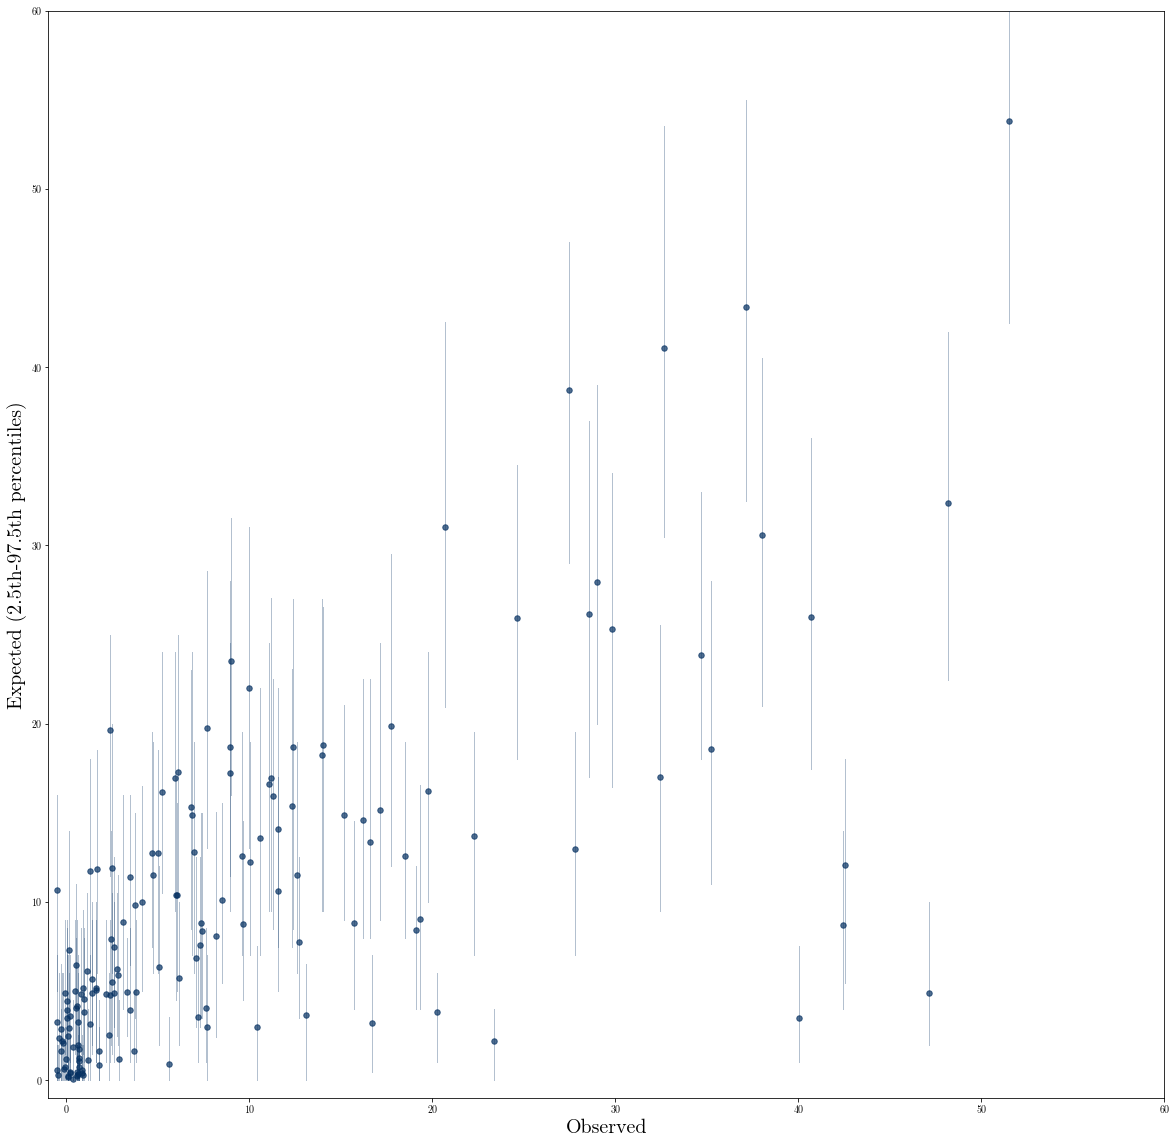
\includegraphics[width=0.75\textwidth]{figures/correlation-percentiles}
	\caption{\textbf{Expected and observed number of dropped samples attaching to each branch in pruned tree.}
	Number of dropped samples actually attached to each branch for pruned simulated Tree 1 plotted against the aggregated number expected by using the coalescent algorithm. Each data point corresponds to a branch in the pruned tree and the intervals around the expected number of dropped samples correspond to the 2.5th and 97.5th percentiles of the expectation created from bootstrapped estimates.
	}
	\label{F-corr}
\end{figure}

\tab Correlation coefficients provide a quantitative measure of overall performance, however, qualitative visualizations are also useful to determine the distribution and rate of attachment along the tree. Figure \ref{F-obs-exp} provides a visual comparison between how many samples are expected to attach at each branch versus how many are actually observed to attach at each branch. Alternatively, instead of raw attachment numbers, we can observe the attachment rate -- number of attachments per unit of branch -- along each branch in Fig. \ref{F-rates}. Expected rates of attachment could provide insight into nearby missed samples and give a measure of amount of attachment that allows direct comparison between branches.

\begin{figure}[h]
 \centering
	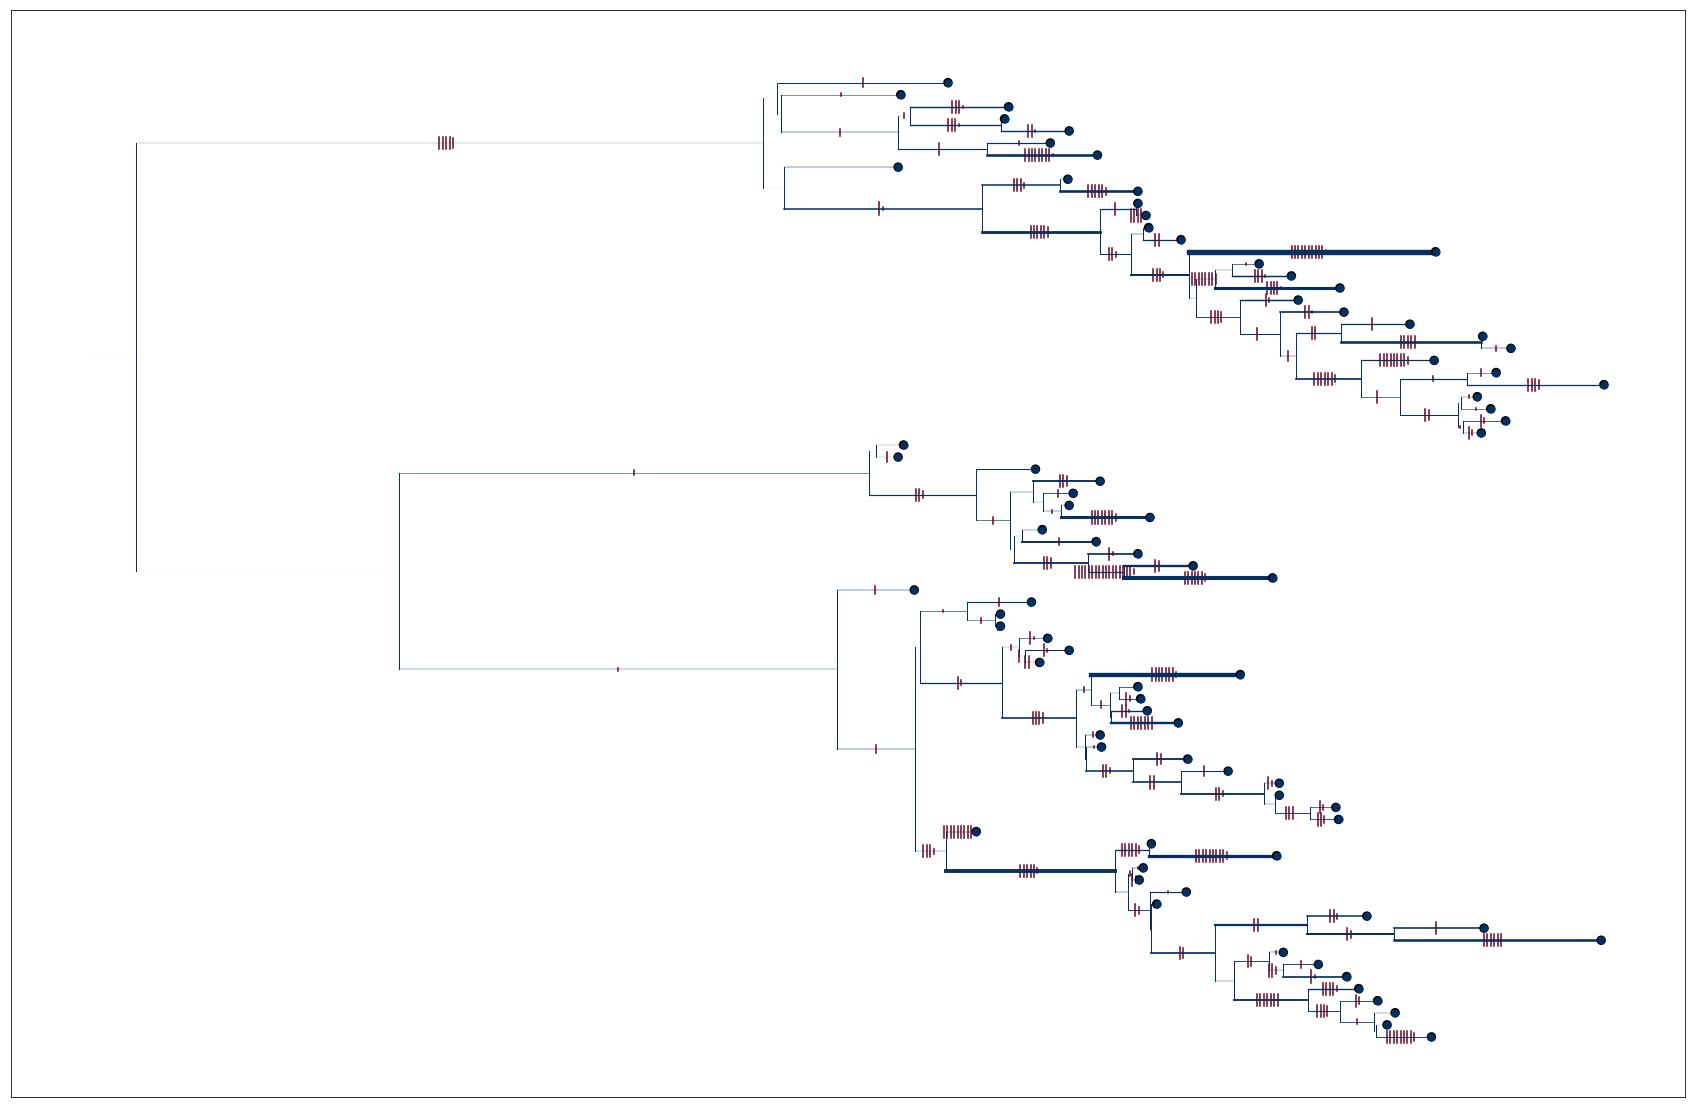
\includegraphics[width=0.75\textwidth]{figures/obs-exp}
	\caption{\textbf{Pruned Tree 1 with overall expected and observed sampling.}
	 Distribution of data observed and expected along example pruned Tree 1. Attachments for the remaining full tree are known. The number of actual dropped samples along each branch are represented by red tick marks where each full tick mark denotes five dropped samples. Partial tick marks are any remaining when the total dropped samples along a branch is not divisible by five. The width of the branch corresponds to the number of predicted samples attaching to a branch where thicker branches represent greater number of expected samples. 
	}
	\label{F-obs-exp}
\end{figure}

\begin{figure}[h]
 \centering
	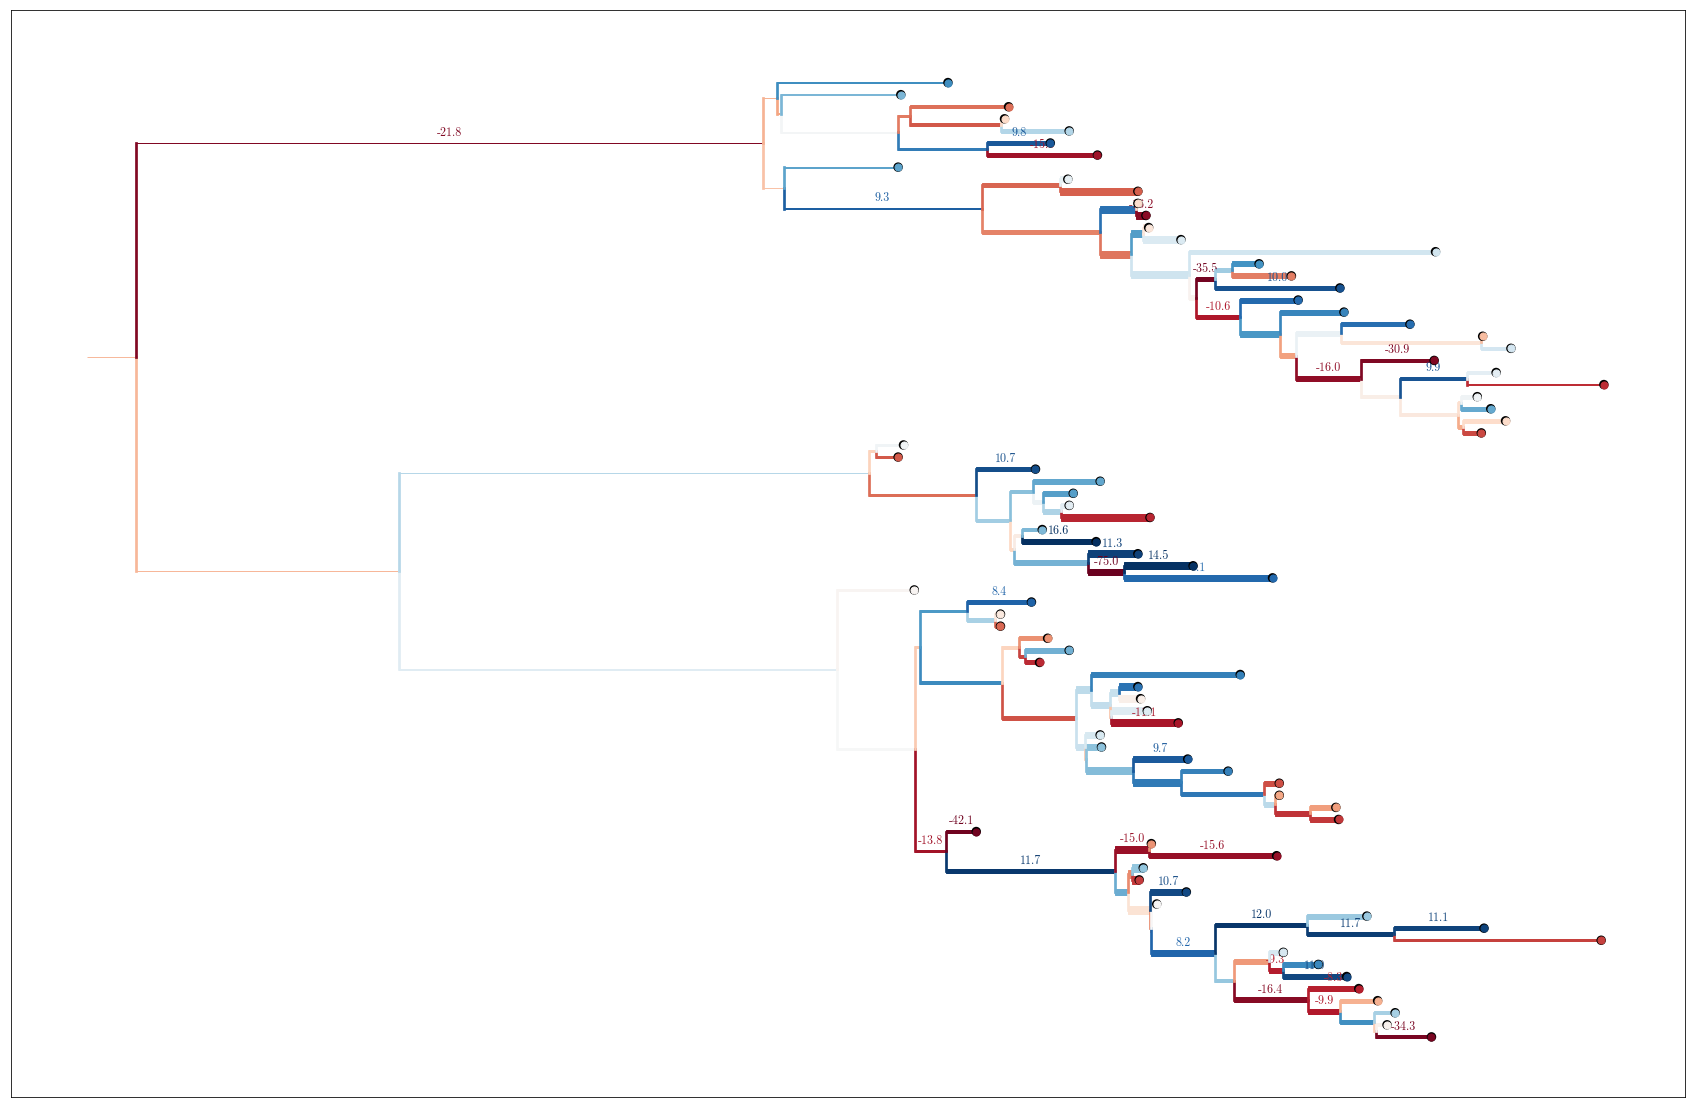
\includegraphics[width=0.75\textwidth]{figures/rate-diff}
	\caption{\textbf{Pruned Tree 1 with expected attachment rates.}
	Example pruned Tree 1 created from a sample of simulated Ebola data. Each branch is colored by the difference between aggregated observed attachments and expected attachments. Darker red corresponds to greater observed than expected and darker blue corresponds to greater expected than observed. Differences greater than .5\% of samples are labeled. The area of the branch is proportional to the number of expected attachments. As a result, the width of the branch represents the ratio of attachments per unit of length, the rate of attachment.
	}
	\label{F-rates}
\end{figure}


%\subsection*{Model Performance Under other Population Models}
% how well does the model perform when assumptions about the population are not fulfilled?
%second table with model performance of other modesl birth death, exponential coalescent



\subsection*{Applying the Coalescent Framework to Ebola Virus Data Set}
%Repeat tip dropping, calculating expectation, and validation on the full ebola tree


%Maybe also Zika 

%% DISCUSSION
\section*{Discussion}


%% METHODS
\section*{Methods}

\subsection*{Data}
\tab The full data consist of 1,610 Ebola virus genome sequences of the Makona variant sampled in Guinea, Sierra Leone, and Liberia from 17 March 2014 to 24 October 2015. The maximum clade credibility (MCC) tree containing the 1,610 sequences was taken from Dudas, et. al.(2017)\cite{dudas2017virus}. 

\tab In addition to the full MCC tree, we also used the Ebola virus samples for simulation and model validation. We used the software BEAST \cite{drummond2007beast} to produce a set of phylogenetic genealogies from the original Ebola virus samples. Instead of using genetic distance to inform genealogy, the samples were treated as empty alignments with no geographic information and allowed to branch based on the standard coalescent framework with a constant population size. From a set of simulated $100,000,000$ genealogies, every $10,000^{th}$ was sampled. From the last 90\% of the sampled trees, five random trees were chosen for model evaluation.

\subsection*{Validation}
\tab Model performance is determined by how well the model can predict attachment of a new sample at a given time to the correct branch. From each of the five simulated trees, 95\% of the samples are randomly dropped and the pruned tree -- consisting of the remaining 5\% or 161 tips -- is kept as the starting genealogy. We chose a sampling proportion of 5\% which reflects the estimated sampling proportion of the actual outbreak \cite{world2016ebola}. Given the time at which each unknown sample was collected, we calculate the probability that each dropped sample attaches to each branch in the pruned tree. These expectations are stored in a matrix where each row corresponds to a dropped sample, the columns denote the branches in the pruned tree, and the cell value corresponds to the probability of attachment for the $i^{th}$ sample to the $j^{th}$ branch. A binary observed matrix marks actual attachment to each branch in the pruned tree. 

\subsection*{Evaluating Sample Specific Model Performance}
\tab Model error is measured by the categorical cross-entropy between the observed attachments and the distribution of attachment expectations for each dropped sample. This is given by
\begin{equation}
	H(p,q) = - \sum_{i=0}^r p_i \cdot log(q_i)
\end{equation}
where $p$ corresponds to the one hot encoding of our known, observed attachments and $q$ is the expected distribution calculated across the $r$ branches remaining in the pruned tree for the $i^{th}$ dropped sample. 

\tab The first benchmark for performance, Null Model 1, is constructed by assigning an equal expectation of attachment to each branch in the pruned tree for each dropped sample. The second benchmark is Null Model 2, another null model where, instead of equal opportunity to attach to each branch, equal opportunity is given to attach to each place in the tree. The probability of attaching to a branch is the individual branch length over the aggregated length of all branches across the tree. In this model, the probability of attaching beyond the root is assumed to be negligible. Longer branches are prioritized as candidates for attachment over shorter ones because they represent a greater proportion of the total sum of branch lengths. The total and average per sample entropy scores resulting from these two null models allow a direct comparison of performance with the our model created under the coalescent framework. 

\newpage
\bibliographystyle{plos}
\bibliography{unsampled}

\end{document}
